\section{Proposed approach}

\subsection{Generative Adversarial Networks}
    We use Generative Adversarial Networks (GANs) to replace the sharpness loss.
    In the GAN framework, there are two models, a generator and a discriminator, that compete against each other in a zero-sum game.
    The goal is to train the generator to generate data when given a dataset, in an unsupervised learning setting.
    The discriminator has to distinguish between the generator's outputs and the data points from the dataset.
    At convergence, we expect the generator to be able to successfully fool the discriminator by learning to generate data that is indistinguishable from the dataset.

    \paragraph{Patch discriminators}
    \citet{pix2pix} extend GANs to also work in supervised learning settings, by introducing the concept of a `patch discriminator'.
    As opposed to traditional GANs, where the discriminator outputs predictions for whole images, the patch discriminator outputs predictions for each $P \times P$ patch of the input image.
    This complements the supervised learning objective to generate more realistic output images.
    As the authors point out, the supervised loss will capture the low-frequency features in the output data, while the discriminator will capture the high-frequency features.

\subsection{Sharpness loss}
    Since we already have a supervised loss for the outputs ($\mathcal{L}_F$), we use a patch discriminator for the sharpness loss.
    The main model is now viewed as a generator.
    The discriminator $D_S$ is a CNN that takes as input an RGBA image $R \in \mathbb{R}^{H \times W \times 4}$ with the same structure and representation as the outputs of the generator.
    It will output a scalar prediction for each $P \times P$ patch in the image, which are averaged to get the output for the entire image.
    The new architecture is shown in Figure~\ref{fig:gan-arch}.

    \begin{figure}
        \centering
        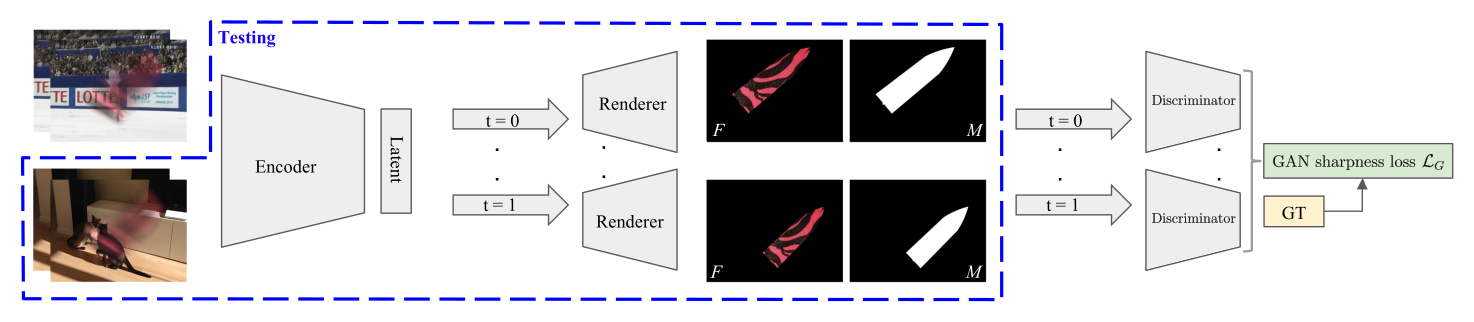
\includegraphics[width=\textwidth]{images/gan-arch.png}
        \caption{
            Architecture for the GAN-based sharpness loss.
            The discriminator takes as input one complete sub-frame and predicts whether each $P \times P$ patch is valid or not.
        }%
        \label{fig:gan-arch}
    \end{figure}

    We use the Wasserstein loss~\citep{wgan} to train the GAN.\@
    This loss requires $D_S$ to be a 1-Lipschitz function.
    We use spectral normalization~\citep{spectral-norm} over all of its weights to enforce this constraint.
    Thus, the new GAN-powered sharpness loss $\mathcal{L}_G$ is:
    \begin{equation}
        \mathcal{L}_G({\{ R_t, \tilde{R}_t \}}_1^N) = \frac{1}{N} \sum_{t=1}^N \left( \mathbb{E}_{\tilde{R}_t}[D_S(\tilde{R}_t)] - \mathbb{E}_{R_t}[D_S(R_t)] \right)
    \end{equation}

    Here, the expectation is approximated by a mean over a batch of inputs.
    The objective for $D_S$ is to maximize this loss, whereas the generator has to minimize this.

    Intuitively, $D_S$ will focus on the high-frequency features of each sub-frame $R_t$ --- both the foreground $F_t$ and the mask $M_t$.
    This means that both the texture of the foreground object and the sharpness of the boundaries must be optimal.
    Since $D_S$ can learn a highly non-linear function, $\mathcal{L}_G$ improves over $\mathcal{L}_S$ in the following ways:
    \begin{itemize}
        \item It incorporates foreground details.
        \item It can identify boundaries and thus relax the constraint of binary mask values near them.
        \item It can enforce spatial continuity of mask values --- entropy has no spatial knowledge.
        \item It is general enough to be used in other tasks involving fine-grained image details.
    \end{itemize}

% TODO: Add/replace with contrastive learning loss
\subsection{Time-consistency loss}
    Here, we modify the objective for the discriminator to distinguish between consecutive frames and random frames.
    The input to this discriminator $D_T$ is a pair of RGBA images $R_1, R_2 \in \mathbb{R}^{H \times W \times 4}$ with each RGBA image having the same structure and representation as the outputs of the generator.
    $D_T$ is a CNN that will be given all possible pairs of output sub-frames, and it has to identify if $R_2$ immediately follows $R_1$.

    Therefore, if either all sub-frames are identical or lack temporal smoothness, then the discriminator cannot distinguish them.
    The only optimum is to have proper temporal smoothness.
    Thus, this loss improves over the previous time-consistency loss since it enforces smooth movement, whereas the previous loss encourages static sub-frames.
    Further, unlike the GAN sharpness loss, this is a self-supervised setup that doesn't need any ground-truth.

    However, unlike the sharpness loss, we cannot use the GAN framework here.
    This is because we want \textbf{both} the discriminator and the generator to optimize this.
    Since the two networks need to help each other, this is not a GAN.\@
    Therefore, we simply model this loss using binary cross-entropy:
    \begin{equation}
        \mathcal{L}_N = - \frac{1}{N^2} \sum_{t=1}^N \sum_{u=1}^N \left( \mathbbm{1}[u=t+1] \log D_T(R_t, R_u) + \mathbbm{1}[u \neq t+1] \log (1 - D_T(R_t, R_u)) \right)
    \end{equation}

    % TODO: Maybe explain perceptual losses?
    This is a novel loss function that can be thought of as a neural-network-based learned loss.
    The architecture for this setup is shown in Figure~\ref{fig:temp-nn-arch}.

    \begin{figure}
        \centering
        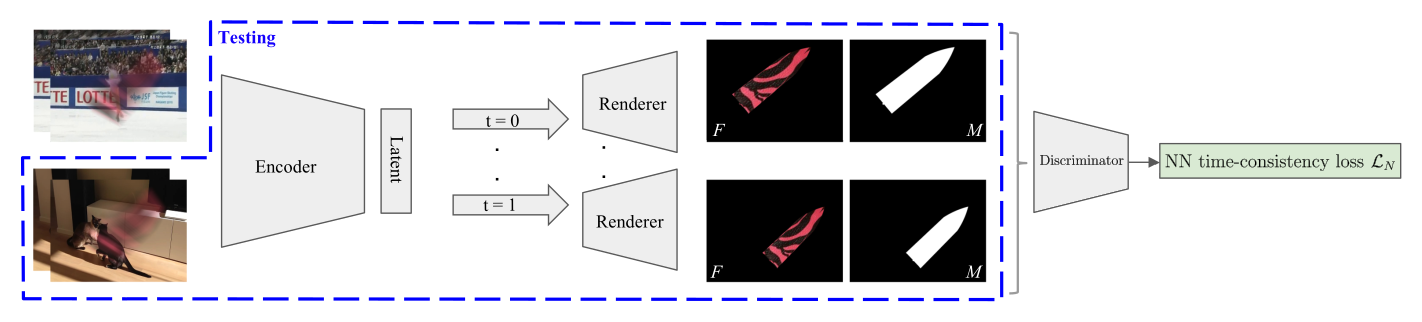
\includegraphics[width=\textwidth]{images/temp-nn-arch.png}
        \caption{
            Architecture for the NN-based time-consistency loss.
            The discriminator takes as input each possible pair of sub-frames separately and predicts whether the second one follows the first.
        }%
        \label{fig:temp-nn-arch}
    \end{figure}

\subsection{Updated Loss}
    Using both the updated sharpness loss ($\mathcal{L}_G$ instead of $\mathcal{L}_S$) and the updated time-consistency loss ($\mathcal{L}_N$ instead of $\mathcal{L}_T$), we change the total loss to:
    \begin{equation}
        \mathcal{L}_{\mathrm{ours}} = \mathcal{L}_F + \alpha_I \mathcal{L}_I + \alpha_N \mathcal{L}_N + \alpha_G \mathcal{L}_G + \alpha_L \mathcal{L}_L
    \end{equation}
